\documentclass[12pt]{article}
\usepackage{scrtime} % for \thistime (this package MUST be listed first!)
\usepackage[margin=0.75in]{geometry}
\usepackage{graphicx}
\usepackage{fancyhdr}
\usepackage{caption}
\usepackage{subcaption}
\usepackage{xspace}
%\usepackage{underscore}
\usepackage{pdfpages}
\usepackage{xcolor,colortbl}%for changing cell colour
\usepackage{longtable}
\usepackage{hyperref}
\usepackage{booktabs}
\usepackage{array}
\pagestyle{fancy}
\setlength{\headheight}{15.2pt}
\setlength{\headsep}{13 pt}
\setlength{\parindent}{28 pt}
\setlength{\parskip}{12 pt}
\pagestyle{fancyplain}
\usepackage[T1]{fontenc}
\usepackage{tikz-cd}
\usepackage{tikz}
\usepackage[normalem]{ulem} %to strikeout text
\usetikzlibrary{decorations.markings}
\usetikzlibrary{calc, arrows}
\usepackage{lscape} %to make the page landscape
\usepackage{color,amsmath,amssymb,amsthm,mathrsfs,amsfonts,dsfont}
\usepackage{indentfirst} % to indent the first paragraph
\rhead{\fancyplain{}{Thesis Update \today \hfill Daniella Lato}}
%\rhead{\fancyplain{}{Thesis Update April 8, 2019 \hfill Daniella Lato}}
\title{Sinorhizobium Update}
\author{Daniella Lato}
\date{\today}
\renewcommand\headrulewidth{0.5mm}
\newcommand{\cc}{\cellcolor{black!16}}
\newcommand{\s}{\textit{Sinorhizobium}\xspace}
\newcommand{\smel}{\textit{S.\,meliloti}\xspace}
\newcommand{\smed}{\textit{S.\,medicae}\xspace}
\newcommand{\sfred}{\textit{S.\,fredii}\xspace}
\newcommand{\ssah}{\textit{S.\,saheli}\xspace}
\newcommand{\ster}{\textit{S.\,terangae}\xspace}
\newcommand{\agro}{\textit{A.\,tumefaciens}\xspace}
\newcommand{\escoli}{\textit{Escherichia coli}\xspace}
\newcommand{\bur}{\textit{Burkholderia}\xspace}
\newcommand{\vib}{\textit{Vibrio}\xspace}
\newcommand{\sul}{\textit{Sulfolobus}\xspace}
\newcommand{\ent}{\textit{Enterobacteria}\xspace}
\newcommand{\p}{progressiveMauve\xspace}
\newcommand{\bas}{\textit{Bacillus subtilis}\xspace}
\newcommand{\strep}{\textit{Streptomyces}\xspace}
\newcommand{\bass}{\textit{B.\,subtilis}\xspace}
\newcommand{\ecol}{\textit{E.\,coli}\xspace}
\newcommand{\ecoli}{\textit{Escherichia coli}\xspace}
\newcommand{\tub}{\textit{Mycobacterium tuberculosis}\xspace}
\newcommand{\pa}{pSymA\xspace}
\newcommand{\pb}{pSymB\xspace}
\newcommand{\snat}{\textit{S.\,natalensis}\xspace}
\newcommand{\scoe}{\textit{S.\,coelicolor}\xspace}
\newcommand{\borrb}{\textit{Borrelia burgdorferi}\xspace}
\providecommand{\e}[1]{\ensuremath{\times 10^{#1}}}
\newcommand{\ch}{$\checkmark$}
\newcommand{\dn}{\textit{dN}\xspace}
\newcommand{\ds}{\textit{dS}\xspace}
\newcommand{\sven}{\textit{S.\,venezuelae}\xspace}
%\newcommand{\scoe}{\textit{S.\,coelicolor}\xspace}
\newcommand{\sliv}{\textit{S.\,lividans}\xspace}
\newcommand{\bor}{\textit{Bordetella}\xspace}
\newcommand{\xan}{\textit{Xanthomonas}\xspace}
\begin{document}
%	Nov 30:	Create graphs with slopes for each COG
	
	
%	Dec 3:	Create new binned scatter plot of COG log reg
	
%	Dec 6:	Determine if there are any other stats I want/need for COG stuff
	
%	Dec 10:	Calculate above stats and write in table
	
%	Dec 21:	Find papers on COG stuff (for intro and discussion), and other mol trends (discussion for sub paper)
	
%	Jan 6:	Read above mentioned papers and make notes
%	Oct 31: Write out methods for gene expression paper
%	
%	Sep 9: Think about/compile list of inversions in \ecol for new paper
%	
%	Nov 15: Think about how to better look at the COG data
%	
%	Nov 25: Complete any extra analysis needed for Substitution paper
%	
%	Dec 4: Mac Scholarships and Awards Due
%	
%	Dec 1: Write out COG methods
%	
%	Dec 15: Gather papers for COG paper intro
%	
%	Dec 15: Implement COG stuff
%	
%	Other things to do:
%	
%	Create outline for gene expression paper
%
%  research mito increased subs near origin
%
%  add above to subs paper writeup
%	
%	Write Write Write gene expression paper
%	
%	 Have gene expression/inversion data combined and in graphical format/regression lines calculated
%	
%	re-do gene exp/sub graphs with patchwork R package so they line up exactly
%	
%	Have data for other molecular trends (GC content, number of genes, essential gene lists..etc.) combined with graphs (or in supplement) for sub analysis
%
% organize all the notes I made for comps into topics that can be integrated into an intro if needed
%	
%	May 31:	Complete COG analysis
%	
%	Jun 30:	COG analysis Paper draft completed
%	
%	Jul 31: Add other mol trends to Sub Paper

\underline{Subs Paper Things to Do:}
\begin{itemize}

%	\item Or get 1st, 2nd, 3rd codon pos log regs

%    \item \sout{why does sinoC have omega lin reg = 0 near and far from the origin?}
%    
 %   \item create new graphs for selection analysis
%    
	\item why are the lin reg of \dn, \ds and $\omega$ NS but the subs graphs are...explain!

	\item mol clock for my analysis?
	
	\item GC content? COG? where do these fit?
	
\end{itemize}

\underline{Inversions and Gene Expression Letter Things to Do:}
\begin{itemize}
%	\item \sout{get as much GEO data as possible}
%	\item \sout{find papers about inversions and expression}
%	
%	\item \sout{see how many inversions I can identify in these strains of \ecoli with gene expression data}
%	
%	\item \sout{read papers about inversions}
%	
%	
%	\item \sout{check if opposite strand in \p means an inversions (check visual matches the xmfa)}
%	
%	\item \sout{check if PARSNP and \p both identify the same inversions (check xmfa file)}
	\item \sout{create latex template for paper}
%	\item \sout{put notes from papers into doc}
%	\item \sout{use large PARSNP alignment to identify inversions}

	\item confirm inversions with dot plot
	\item make dot plot of just gene presence and absence matrix (instead of each site) to see if this will go better
	\item look up inversions and small RNA's paper Marie was talking about at Committee meeting
	\item write outline for letter
	\item write Abstract
	\item \sout{write intro}
	\item write methods
	\item compile tables (supplementary)
	\item write results
	\item write discussion
	\item write conclusion 
	\item do same ancestral/phylogenetic analysis that I did in the subs paper 
\end{itemize}

\underline{General Things to Do:}
\begin{itemize}
	\item summarize references 40 and 56 from Committee meeting report (Brian was asking)
	
	
\end{itemize}


% next week look into how to calculate the dN/dS for the subs paper
% week of Dec 17th do same ancestral analysis on gene exp data for ecoli...which is going to require me to do everything from scratch so make a tree and all that jazz

	
\section*{Last Week}
Substitutions Paper:
\ch looked over reviewers comments

\ch started the ``leave one out'' analysis

Inversions $+$ Gene Expression:

\ch Queenie finished final dataframes!

\ch wrote code to get non-coding positions

\ch obtain new inversion combos for DESeq

\ch final aesthetic inversions and expression graph

General:

\ch Wrote 3pages for conclusion of Dissertation

\bigskip

\textbf{Inversions + Gene Expression:}

\textbf{Final dataframes:}
Queenie has finished the final dataframes for this analysis for both the raw data (for DESeq) and normalized expression values (for other analysis).
I am in the process of looking these over to double check that everything is correct.
So far it looks like we had about 1000 genes that were aligned with PARSNP but were not reciprocal best BLAST hits, leaving us with a total of just over 2000 genes to analyze.


\textbf{Non-coding H-NS data:}
I started to combine information from the coding and non-coding H-NS binding data and had to write some code to obtain the genomic position for one datasets as it only told me the flanking genes.
I am still working on combining all non-coding information with the coding information for all H-NS binding datasets.

\textbf{Inversion Combos:}
DESeq requires ``treatment'' information for each sample so I have obtained all of the different inversion combinations that exist in our raw data frame (i.e. inversion in only ATCC, or ATCC and DH, ...etc).

\textbf{Inversions and Expression Graph:}
I have finished tweaking the final aesthetics for Figure \ref{fig:inver_exp}.
Let me know if you think there is anything I should add or change.
I still need to run this through using Queenie's final dataframes.
In this graph I chose to only use the genomic position for K12 MG1655 to represent the singular position for each block.
Trying to account for varying positions in each taxa was too messy graphically.
\textbf{Do you think it is appropriate to use only K12 MG1655 positions? My thought was that this would be sort of the ``reference'' and then I could do regressions on each strain separately to see if/how inversions vary with distance from the origin of replication. Thoughts?}



\textbf{Inversion Visualization:}
I did not get a chance to look into the output from the two inversion visualization figures (with and without ATCC reverse complemented) (Figures \ref{fig:inversion_norevcomp} and \ref{fig:inversion_revcomp}).
I will look into these more this week.
%I have been looking at programs to best depict the inversions we are seeing but most take too long to run (dot plots) or are quite complicated in the input files.
%I found a way to use parallel sets in \texttt{R} to get around this and I think they are pretty good (Figure \ref{fig:inversion_norevcomp})!
%In Figure \ref{fig:inversion_norevcomp}, it appears as though the whole ATCC genome (CP009072) is inverted.
%So I decided to reverse complement the entire genome of ATCC and then re-create the diagram to see if it would make a difference (Figure \ref{fig:inversion_revcomp}).
%Figure \ref{fig:inversion_revcomp} does clean things up a bit and still shows some of the inversions.
%Additionally, I am a bit confused because theoretically just reversing one sequence should still identify the same blocks in \texttt{PARSNP} when the sequence is not reversed.
%However, the blocks are all slightly different in their positions but the overall \texttt{PARSNP} visualization looks identical.
%So I am a bit confused about which image I should use in the paper.
%My main concern with this is if it is ok to use one image for the visualization (the reverse complemented image Figure \ref{fig:inversion_revcomp}), and the data from the other figure (non-reverse complemented Figure \ref{fig:inversion_norevcomp}) for the data analysis.
%I mention this because when ATCC is reverse complemented it complicates the genomic position annotation. So I would have to ensure that all my annotation is also reverse complemented and that I am grabbing the correct sequence (reverse of the reverse complement?) when I re-align with \texttt{MAFFT}.
%\textbf{What are your thoughts on this?}



%I also noticed from Figures \ref{fig:inversion_norevcomp} and \ref{fig:inversion_revcomp} that a lot of the inversions have been rearranged in addition to being inverted.
%I am not sure how best to account for this in my calculations.
%\textbf{Do you have any thoughts on this?}

\textbf{Substitutions Paper:}

I started to run the ``leave one out'' analysis on \ecol and I will let you know the results once they come in!

I looked at the reviewers comments once again and I agree that Reviewer 2 is concerned about how robust our analysis is.
They want to know if the differences in sign for the substitution correlation is due to i) the small sample size, ii) actual differences/the rearrangements and what we are claiming, or iii) differences between the datasets, I think meaning we see negative in \ecol because rather than \strep because of those particular sequences we chose.
It seems as though they want one of the following things to be done:
\begin{enumerate}
	\item do my analysis (and pipeline) on the same genomes that previous papers used. to show that with our pipeline we get varying signs in our correlations
	\item somehow do my analysis without accounting for rearrangements. This way we can show that without rearrangements we get the same increasing trend as previous studies, but with rearrangements we do not.
\end{enumerate}

We have discussed option 1) a few times and concluded that it just does not make sense to re-do my analysis when the genome annotation has likely changed on these previous datasets since they were published.
I was thinking about option 2) a bit more and I thought of maybe just cutting out the ancestral reconstruction part of my analysis and only looking at the substitutions we see in the extant taxa and their associated genomic positions.
However, since I did my alignment with \p the genomic positions of these extant sequences already has some component of genomic rearrangement accounted for.
So I am wondering if I should re-do the whole genome alignments with a different alignment program?
\textbf{What do you think about all this? Do you think I should do this analysis? If so, do I need to align the genomes with another program?}

%%%%%%%%%%%%%%%%%%%%%%%%%%%%
% HOW LARGE CAN THE SLOPE GET JUNE 1 2020
%%%%%%%%%%%%%%%%%%%%%%%%%%%%
%I also did the test for looking at the substitutions slope and how large it can be.
%I did this by taking the largest non-outlier bar (weighted total substitutions/10Kbp) and set the position to 0, then making another fake point with position at the terminus and a substitutions value of 0, then computing a regression.
%The results can be found in Table \ref{tab:bigslope} and the actual slope values can be found in Table \ref{tab:cod_non_cod_log_reg}.
%The slopes still seem very small to me. \textbf{What do you think? How should I approach this accurately in the paper?}
%
%\begin{table}[h]
%	\centering
%	\resizebox{0.5\textwidth}{!}{%
%		\begin{tabular}{ll}
%			\toprule
%			Bacteria and Replicon &  Test Regression slope \\
%			\midrule
%			\ecol Chromosome & -2.94\e{-9} \\
%			\bass Chromosome &  -5.08\e{-9}\\
%			\strep Chromosome & -3.92\e{-10}\\
%			\smel Chromosome & -3.32\e{-10}\\
%			\smel pSymA & -5.66\e{-9} \\
%			\smel pSymB &  -5.65\e{-9}\\
%			\bottomrule
%		\end{tabular}
%		
%	}%resizebox
%	\caption{\label{tab:bigslope} Values of regression slope for each replicon using two points: 1) Highest weighted value of the number of substitutions / 10Kbp at position zero and 2) weighted value of the number of substitutions / 10Kbp of zero at the terminus. Simple linear regression was calculated. All results have no residuals (no residual degrees of freedom) because there are only two points on the line.}
%\end{table}



%I created a new theme for the selection and substitution graphs so that they all look relatively the same (similar margins, font size..etc).
%Last week when I was re-doing the SH-Test (to see which block trees were different from the overall tree), I realized that some of these blocks were not removed from the analysis in \ecol, \smel Chromosome and \pa.
%I spent most of this week re-running these analysis with the correct number of blocks.
%The new figures and results can be found below and in the attached Supplementary File for the paper. Nothing has changed significantly.
%\smel chromosome looks really terrible. All non-outlier points for \dn and $\omega$ are zero values. Therefore a regression is pointless and makes the selection graph look really odd.
%I started to look into this but it looks like the \smel chromosomes are just so similar that there are hardly any substitutions.
%This is particularly evident when you look at the backbone of the \p alignment (which shows similar sequences).
%When looking at the \ecoli alignement (Figure \ref{fig:ecoli_mauve}) we see that the backbone is very ``spiky'' indicating regions where the nucleotides are not similar.
%The same can be said for the \strep genomes (Figure \ref{fig:strep_mauve}), even though these are more similar to each other than the \ecoli genomes. 
%When we look at the \smel Chromosome alignment (Figure \ref{fig:sinoC_mauve}), we see that the backbone is almost completely flat, meaning that there is hardly any variation in the nucleotide sequence.
%This is especially curious because there appears to be no different in the average number of substitutions in the \smel chromosome (Table \ref{tab:avg_subs}).
%It could be that all the variation is being considered an ``outlier'' because most of the values are zero (because they are so smilar)?
%I am still really confused about why the selection graph for \smel Chromosome looks so odd and the only explanation I can come up with is that the sequences are just really really similar. \textbf{Do you have any thoughts on this or suggestions for other things I could investigate to figure out what is going on?}



\section*{This Week}
%aim to tick off 4 tasks a week
%
\begin{itemize}
	\item double check Queenie's final dataframes 
	\item double check new inversion combos with Queenie's new data frames
\item get previous code working with Queenie's new dataframes
\item combine/read in all data from all H-NS coding and non-coding datasets
\item write code to compare all H-NS datasets to inversions 
\item summarize $\uparrow$ results
\item look into differences between inversion visualization with and without ATCC reverse complemented
\item continue to run the ``leave one out'' analysis on subst data

\end{itemize}


\section*{Next Week}
\begin{itemize}
	\item actual analysis on DESeq data
	\item visualizations/results for $\uparrow$
	\item read papers on H-NS proteins
	\item think about how to visualize H-NS and inversions info
	
	\item continue to run the ``leave one out'' analysis on subst data
\end{itemize}

\newpage

\begin{figure}
	\includegraphics[width=\textwidth]{C:/Users/synch/Documents/PhD/inversion_and_gene_exp_work/Inversion_viz/parallel_sets_all.pdf}
	\caption{\label{fig:inversion_norevcomp} Visualization of rearrangements and inversions in all \ecol strains. ATCC is in the GenBank listed orientation.}
\end{figure}

\begin{figure}
	\includegraphics[width=\textwidth]{C:/Users/synch/Documents/PhD/inversion_and_gene_exp_work/Inversion_viz/parallel_sets_all_ATCC_revcomp.pdf}
	\caption{\label{fig:inversion_revcomp} Visualization of rearrangements and inversions in all \ecol strains. ATCC is reverse complemented from the GenBank listed orientation.}
\end{figure}

\begin{figure}
	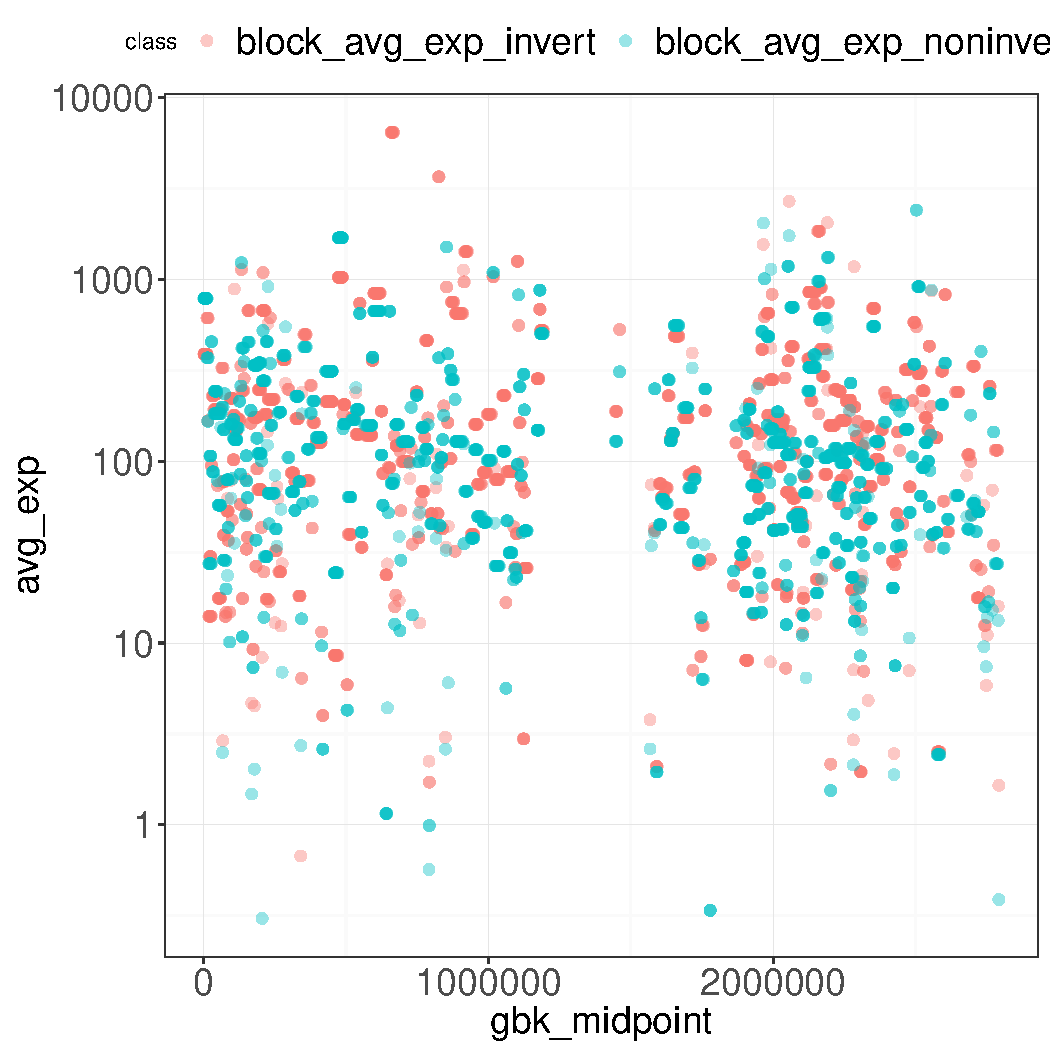
\includegraphics[width=\textwidth]{C:/Users/synch/Documents/PhD/Thesis_Update/genome_pos_inversions_k12.pdf}
	\caption{\label{fig:inver_exp} Visualization of the difference in gene expression between inverted and non-inverted sequences within alignment blocks. Each alignment block represents homologous sequences between the \ecoli strains \textcolor{red}{insert table ref here}. Each alignment block has one point on the graph to represent the average expression value in \textbf{C}ounts \textbf{P}er \textbf{M}illion (\textbf{CPM}) for all inverted (circles) and non-inverted (triangles) sequences within the block. Blocks that had a significant difference in gene expression (using a Wilcoxon sign-ranked test, see Materials and Methods) have the inverted and non-inverted gene expression averages highlighted in pink circles and purple triangles respectively. A smoothing line (\texttt{loewss}) was added to link the average gene expression values for the inverted (pink solid) and non-inverted (purple dashed) sequences within block that had a significant difference in gene expression (using a Wilcoxon sign-ranked test, see Materials and Methods). All blocks that did not have a significant difference in average gene expression between inverted and non-inverted sequences within alignment blocks have the average inversion (circles) and non-inversion (triangles) gene expression values coloured in light grey.}
\end{figure}


\begin{table}[h]
	\centering
	\resizebox{\textwidth}{!}{%
		\begin{tabular}{lcc}
			\toprule
			H-NS Binding Study & All Inversions and H-NS Binding & Significant Inversions and H-NS Binding \\
			\midrule
			Grainger 2006 & NS & NS \\
			Ueda 2013 &  NS & NS \\
			Higashi 2016: coding criteria 1 & 0.102*& 0.101***\\
			 Higashi 2016: coding criteria 1 & 0.101* & 0.089***\\
			and non-coding criteria 1 & & \\
			Higashi 2016: coding criteria 1 & 0.101* & 0.089***\\
			and non-coding criteria 2 & & \\
			Higashi 2016: coding criteria 1 & 0.101* & 0.089***\\
			and non-coding criteria 3 & & \\
			Higashi 2016: coding criteria 2 & 0.104* & 0.090***\\
			Higashi 2016: coding criteria 3 & 0.104* & 0.090***\\
			\bottomrule
		\end{tabular}
		
	}%resizebox
	\caption{\label{tab:HNS} Pearson correlation between H-NS binding sites and inverted regions of the \ecol K-12 MG1655 genome. A genomic region was considered inverted if this sequence was inverted in any of the following four taxa: \ecol K-12 MG1655, \ecol K-12 DH10B, \ecol BW25113, and \ecol ATCC. The genomic positions of these inversions in \ecol K-12 MG1655 was used for reference. The binding sites for the H-NS protein are in the genomic coordinates of \ecol K-12 MG1655, chosen as a reference. The second column ``All Inversions and H-NS Binding'' represents the correlation coefficient between inverted regions and H-NS binding sites. The third column ``Significant Inversions and H-NS Binding'' represents the correlation coefficient between inverted regions with significant differences in normalized gene expression between inverted and non-inverted taxa (via a Wilcoxon signed-rank test) and H-NS binding sites. All results are marked with significance codes as followed: $<$ 0.001 = `***', 0.001 $<$ 0.01 = `**', 0.01 $<$ 0.05 = `*', $>$ 0.05 = `NS'.}
\end{table}

\begin{table}[t!]
	\centering
	\resizebox{\textwidth}{!}{%
		\begin{tabular}{lc}
			\toprule
			Datasets:  & Correlation Coefficient (W)\\
			\midrule
			Inverted Blocks & 15218699**\\
			Inverted Sequences & 11436344***\\
			\bottomrule
		\end{tabular}
	}%resizebox
	\caption{\label{tab:overall_inver_exp} Correlation coefficients for Wilcoxon signed-rank test on various datasets to determine the correlation between an inversion and difference in normalized gene expression. The ``Inverted Blocks'' dataset represents alignment blocks that have at least one taxa with an inverted sequence. The ``Inverted Sequences'' dataset represents all individual sequences from all alignment blocks that were inverted. The correlation between both datasets was computed using a Wilcoxon signed-rank test. All results are marked with significance codes as followed: $<$ 0.001 = `***', 0.001 $<$ 0.01 = `**', 0.01 $<$ 0.05 = `*', $>$ 0.05 = `NS'.}
\end{table}


\begin{table}[t!]
	\centering
	\resizebox{\textwidth}{!}{%
		\begin{tabular}{ccc}
			\toprule
			 \multicolumn{3}{c}{\% of Blocks that are}  \\
			\cmidrule{1-3}
			Inverted & Inverted with &Increased in \\
			  & Differences in&Gene Expression\\
			  & Gene Expression & in Inverted Sequences \\
			\midrule
			68.29 & 8.22& 58.06 \\
			\bottomrule
		\end{tabular}
	}%resizebox
	\caption{\label{tab:multi_taxa_inver} Percent of blocks in categories for various datasets (blocks with all 4 taxa, at least 3 taxa, or at least 2 taxa). The second column is any block that had at least one sequences that was inverted. The last column only deals with blocks that had at least one inverted sequence and had a significant difference in gene expression (column 3).}
\end{table}

\begin{table}[t!]
	\centering
	\resizebox{\textwidth}{!}{%
		\begin{tabular}{c}
			\toprule
			Block Length Correlation Coefficient (W)\\
			\midrule
			4060729.5***\\
			\bottomrule
		\end{tabular}
	}%resizebox
	\caption{\label{tab:len_summary} Correlation coefficients for Wilcoxon signed-rank test in alignment blocks. The correlation coefficient represents a correlation between alignment block length and blocks with a significant/non-significant difference in normalized gene expression between inverted and non-inverted sequences within the block. All results are marked with significance codes as followed: $<$ 0.001 = `***', 0.001 $<$ 0.01 = `**', 0.01 $<$ 0.05 = `*', $>$ 0.05 = `NS'.}
\end{table}




\begin{table}[t!]
	\centering
	\resizebox{\textwidth}{!}{%
		\begin{tabular}{c}
			\toprule
			 Genomic Position Correlation Coefficient (W)\\
			\midrule
			 NS\\
			\bottomrule
		\end{tabular}
	}%resizebox
	\caption{\label{tab:pos_summary} Correlation coefficients for Wilcoxon signed-rank test in alignment blocks with a significant difference in normalized gene expression between inverted and non-inverted sequences within the block. Column 1 depicts the correlation coefficient between the significant blocks and the genomic position of the alignment blocks. All results are marked with significance codes as followed: $<$ 0.001 = `***', 0.001 $<$ 0.01 = `**', 0.01 $<$ 0.05 = `*', $>$ 0.05 = `NS'.}
\end{table}

\begin{table}[h]
	\centering
	\resizebox{\textwidth}{!}{%
		\begin{tabular}{lcc}
			\toprule
			Inversion Category & midpoint & gbk midpoint \\
			\midrule
			rev comp & NS & NS \\
			inversion & 2.20\e{-7}***& 2.20\e{-7}*** \\
			sig rev comp & -1.89\e{-7}* & -1.89\e{-7}*\\
			sig ~ midpoint all blocks & NS & NS \\
			sig ~ midpoint inverted blocks & NS & NS \\
% below category makes no sense bc all sig blocks will be labeled as inverted.
%			sig inversion & NS & NS\\
			\bottomrule
		\end{tabular}
		
	}%resizebox
	\caption{\label{tab:log_reg} Logistic regression between various inversion categories and distance from the origin of replication for all strains. rev comp = individual sequences inverted, inversion = block that has at least one inverted sequence, midpoint = block midpoint, gbk midpoint = gene midpoint, sig = blocks with significant difference in normalized gene expression between inverted and non-inverted sequences within the block. All results are marked with significance codes as followed: $<$ 0.001 = `***', 0.001 $<$ 0.01 = `**', 0.01 $<$ 0.05 = `*', $>$ 0.05 = `NS'.}
\end{table}

\begin{table}[h]
	\centering
	\resizebox{\textwidth}{!}{%
		\begin{tabular}{lcc}
			\toprule
			Strain & rev comp & inversion \\
			\midrule
			%K12 and BW have no inverted seqs so they have no values for first col
			%no strains have values for second col because all sig blocks have inversion=1 for all rows
			\ecol K-12 MG1655 &  & 3.55\e{-7}*** \\
			\ecol K-12 DH10B & NS & 3.45\e{-7}*** \\
			\ecol BW25113 & & 3.73\e{-7}***\\
			\ecol ATCC & -1.92\e{-7}*** & -1.92\e{-7}*** \\
			\bottomrule
		\end{tabular}
		
	}%resizebox
	\caption{\label{tab:log_reg_strain} Logistic regression between various inversion categories and distance from the origin of replication for  each strain. rev comp = individual sequences inverted, inversion = block that has at least one inverted sequence, sig = blocks with significant difference in normalized gene expression between inverted and non-inverted sequences within the block. All results are marked with significance codes as followed: $<$ 0.001 = `***', 0.001 $<$ 0.01 = `**', 0.01 $<$ 0.05 = `*', $>$ 0.05 = `NS'.}
\end{table}
\end{document}
